\documentclass[11pt,a4paper]{article}

% These are extra packages that you might need for writing the equations:
\usepackage{amsmath}
\usepackage{amsfonts}
\usepackage{amssymb}
\usepackage{booktabs}
\usepackage{hyperref}
\usepackage{listings}
\usepackage{xcolor}
\lstset {language=C++,
		 basicstyle=\ttfamily,
         keywordstyle=\color{blue}\ttfamily,
         stringstyle=\color{red}\ttfamily,
         commentstyle=\color{purple}\ttfamily,
         morecomment=[l][\color{magenta}]{\#},
       	 basicstyle=\tiny}

% You need the following package in order to include figures in your report:
\usepackage{graphicx}

% With this package you can set the size of the margins manually:
\usepackage[left=2cm,right=2cm,top=2cm,bottom=2cm]{geometry}


\begin{document}

% Enter the exercise number, your name and date here:
\noindent\parbox{\linewidth}{
 \parbox{.25\linewidth}{ \large HPCSE I, Exercise 04 }\hfill
 \parbox{.5\linewidth}{\begin{center} \large Beat Hubmann \end{center}}\hfill
 \parbox{.2\linewidth}{\begin{flushright} \large Oct 22, 2018 \end{flushright}}
}
\noindent\rule{\linewidth}{2pt}

\section{Question 1: Amdahl's Law}

\subsection{Task a)}
Disregarding the misplaced marketing hyperbole for the sake of the argument and assuming the new train route follows the bus route (i.e. has the same length),
 we designate the section from Luzern to Rotkreuz as serial fraction:
$f_1 = \frac{55 \text{km} - 36 \text{km}}{55 \text{km}} = 0.345$. This leaves the potential new train section as improvable fraction: $f_p = 1 - f_1 = 0.655$.
Based on the information given, we assume that the average speed $v_b = \frac{55 \text{km}}{1.5 \text{h}} = 36.67 \text{km/h} $ of the bus 
on the total leg LU-ZH also applies to the fraction $f_1$, whereas $v_t = 70 \text{km/h}$ is given for the train speed on the fraction $f_p$.
This in turn gives a speedup factor $p = \frac{70 \text{km/h}}{36.67 \text{km/h}} = 1.91$.

\subsubsection{Task a.i)}
Nobody will get any improvement from the announcement per se, but if implemented, it will offer a speedup of 1.453 as seen from equation~\ref{eqn:1}.
In other words, the ideal one-way journey time will reduce from 90 minutes to 62 minutes.

\begin{equation}
    S_p = \frac{1}{f_1 + \frac{f_p}{p}} = \frac{1}{0.345 + \frac{0.655}{1.91}} = 1.453
\label{eqn:1}
\end{equation}

\subsubsection{Task a.ii)}
Again using equation~\ref{eqn:1}, this time with a (rounded) speedup factor of $p = 3 \cdot 10^7$, we get a theoretical speedup of 2.9 and thus
a one-way journey time of about 30 minutes.

\subsection{Task b)}
As per the task description, we disregard hyperthreading and thus plainly assume 12 CPU cores per socket. Also, we are given that 
$f_p = 0.9$ and thus $f_1 = 1 - f_p = 0.1$. Finally, we assume that the code currently is in serialized form running on a single core.

\subsubsection{Task b.i)}
The desired speedup is given as $S_p = 8$. Solving equation~\ref{eqn:1} for $p$, 
we get that the desired speedup from serial execution requires a minimum of 36 cores (equation~\ref{eqn:2}).

\begin{equation}
    p = \frac{S_p \cdot f_p}{1 - S_p \cdot f_1 } = \frac{8 \cdot 0.9}{1 - 8 \cdot 0.1} = 36
\label{eqn:2}
\end{equation}

\subsubsection{Task b.ii)}
As we need three full sockets (36 / 12 = 3), but sockets only come paired up as nodes, we require two nodes. As we then might as well
use them completely, the obtainable speed up is, again using equation~\ref{eqn:1}, $S_{p=48} = \frac{1}{0.1 + \frac{0.9}{48}} = 8.42$.

\subsubsection{Task b.iii)}
The price for additional nodes can safely be assumed to be non-negligible. It can therefore credibly be argued that buying more nodes doesn't 
make any sense, as obviously even for $p \rightarrow \infty$ the absolute best obtainable speedup would be
 $\lim_{p \rightarrow \infty} S_p = \frac{1}{0.1 + \frac{0.9}{p}} = 10$.

% \begin{figure}[ht]
% \begin{center}
% 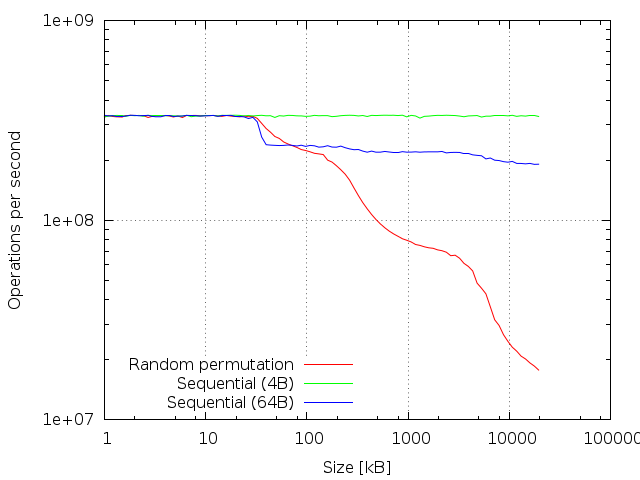
\includegraphics[scale=0.5]{results.png} 
% \end{center}
% \caption{Parallel Monte Carlo integration on Euler compute cluster.}
% \label{fig1}
% \end{figure}

\section{Question 2: Manual Vectorization of Reduction Operator}

Blub

\subsection{Task a)}


\subsection{Task b)}

\subsection{Task c)}

\subsubsection{Task c.i)}
Blub

\subsubsection{Task c.ii)}
Blub


% \begin{figure}[ht]
% \begin{center}
% 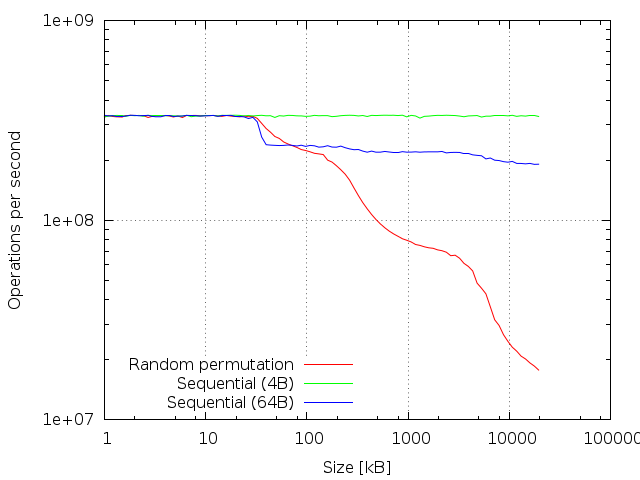
\includegraphics[scale=0.5]{results.png} 
% \end{center}
% \caption{Parallel Monte Carlo integration on Euler compute cluster.}
% \label{fig1}
% \end{figure}

\section{Question 3}

Blub

\subsection{Task a)}


\subsection{Task b)}

\subsection{Task c)}

\subsection{Task d)}

\subsection{Task e)}

\subsection{Task f)}

\begin{lstlisting}[float, caption={Proposed modification for correctness in task 2.}, label={lst1}]
    #pragma omp parallel for
    for (int i= 0; i < N; i++)
    {
        if (is_good(i)) // No change until here
        {
            int thread_pos{0}; // Define thread specific position variable
            #pragma omp critical // This block replaces the #pragma omp atomic section
            {
                thread_pos= pos; // Protected read
                pos++; // Protected write
            }
            good_members[thread_pos]= i; // Use thread specific variable
        }
    }
\end{lstlisting}


%\begin{thebibliography}{99}
%
%\bibitem{nasa}
%	NASA,
%	\emph{Haswell Processors},
%	online (\url{https://www.nas.nasa.gov/hecc/support/kb/haswell-processors_492.html}),
%	accessed 30-Sep-2018.
%
%\bibitem{intel}
%	Intel Corporation,
%	\emph{Intel Xeon Processor E5-2680 v3 Product Specifications},
%	online (\url{https://ark.intel.com/products/81908/}),
%	accessed 30-Sep-2018.
%	
%\bibitem{euler}
%	ETH Zurich,
%	\emph{scientific computing wiki: Euler},
%	online (\url{https://scicomp.ethz.ch/wiki/Euler#Euler_II}),
%	accessed 30-Sep-2018.	
%
%\bibitem{kou}
%	Petros Koumoutsakos,
%	\emph{HPCSE I Lecture Notes},
%	online (\url{http://www.cse-lab.ethz.ch/wp-content/uploads/2018/09/HPCSE_I_1_Intro.pdf}),
%	accessed 30-Sep-2018.
%
%\end{thebibliography}
%

%\appendix
%\section{Question 4, task d)}\label{app}
%\lstinputlisting{ex01_q4_task_d.cpp}
\end{document}